\documentclass[tikz,border=1mm]{standalone}
\begin{comment}
:Title: NORTH-EASTERN HILL UNIVERSITY (NEHU) logo
:Tags: tikz; pgfornament, tikzrput
:Author: LAIRENLAKPAM JOYPRAKASH SINGH, MANIPUR
\end{comment}

% TikZ
\usepackage{tikz, pgfornament, tikzrput}
\usetikzlibrary{decorations, decorations.text}

% font size
\usepackage{fix-cm}

\tikzstyle{periphery}=[draw=black,fill=black]

\begin{document}
\begin{tikzpicture}%[overlay,remember picture]
% outer circle
	\fill[orange!85] (0,0) circle (4.8cm);
		\draw[line width=1.6 mm] circle[radius=4.8cm];
% inner circles1
	\fill[yellow!90] (0,-0.5) circle(2.6cm);
		\draw[line width=1.4 mm] (0,-0.5) circle[radius=2.6cm];
% inner circles2
	\fill[orange!85] (0,-1.5) circle(0.7cm);
		\draw[line width=1.0 mm] (0,-1.5) circle[radius=0.7cm];
% sunlight
	\node at (0,-1.2)[scale=1]{%
		\begin{tikzpicture}%[minimum width=40]
		\node[circle,inner sep=22pt]  at (0,0) (a) {};      
		\foreach \angle in {185,195,...,355}{%
			\draw[line width=0.5mm] (a.-\angle) -- (-\angle:1.6cm);
			}
%		\node[circle]  at (0,0) (a) {}; 
		\foreach \angle in {180,190,...,360}{%
			\draw[line width=0.5mm]  (a.-\angle) -- (-\angle:1.4cm);
			}
		\end{tikzpicture}
	};
% outer text
	\path[%rotate=-15.2,
		postaction={%
			decoration={%
				text along path,%text width=5cm,
				text={%
					|\fontsize{21pt}{2em}\bf\sffamily\selectfont| % any size
						NORTH-EASTERN HILL UNIVERSITY %
					},
				text align=center,%xslant=(0)*3,
				reverse path,
				},
			decorate
			},text effects={scale text to path}
		] (-25:3.4cm) arc (-25:210:3.4cm);  
% Patch behind yellow box
	\fill[orange!85] (-3,-3.6) rectangle (3.0,-2.6);
%
	\node at (-2.6,-2.0)[scale=1]{%
	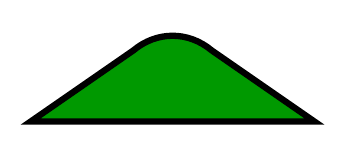
\begin{tikzpicture}
		\draw[fill=green!60!black] (0,0) to (1.3,0.9) 
			to [out=40, in=140] (2.3,0.9) to (3.6,0) to (0,0);
		\draw[line width=0.8mm] (0,0) to (1.3,0.9) 
			to [out=40, in=140] (2.3,0.9) to (3.6,0) to (0,0) to (1.3,0.9);
	\end{tikzpicture}};
	\node at (2.6,-2.0)[scale=1]{%
	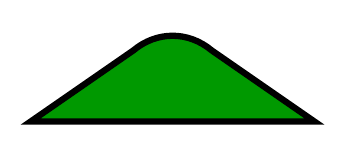
\begin{tikzpicture}
		\draw[fill=green!60!black] (0,0) to (1.3,0.9) 
			to [out=40, in=140] (2.3,0.9) to (3.6,0) to (0,0);
		\draw[line width=0.8mm] (0,0) to (1.3,0.9) 
			to [out=40, in=140] (2.3,0.9) to (3.6,0) to (0,0) to (1.3,0.9);
	\end{tikzpicture}};
%
	\node at (1.0,-2.05)[scale=1]{%
	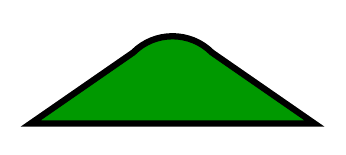
\begin{tikzpicture}
		\draw[fill=green!60!black] (0,0) to (1.3,0.9) 
			to [out=45, in=135] (2.3,0.9) to (3.6,0) to (0,0);
		\draw[line width=0.8mm] (0,0) to (1.3,0.9) 
			to [out=45, in=135] (2.3,0.9) to (3.6,0) to (0,0) to (1.3,0.9);
	\end{tikzpicture}};
%
	\node at (-0.9,-2.08)[scale=1]{%
	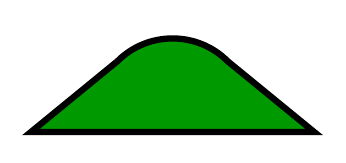
\begin{tikzpicture}
		\draw[fill=green!60!black] (0,0.1) to (1.1,1.0) 
			to [out=45, in=135] (2.5,1.0) to (3.6,0.1) to (0,0.1);
		\draw[line width=0.8mm] (0,0.1) to (1.1,1.0) 
			to [out=45, in=135] (2.5,1.0) to (3.6,0.1) to (0,0.1) to (1.1,1.0);
	\end{tikzpicture}};
% yellow rectangle
	\node at (0,-3.24)[scale=1]{%
	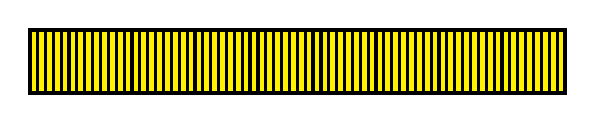
\begin{tikzpicture}%[minimum width=40]
		\draw[fill=yellow, line width=1.4,draw] (0,0) rectangle (6.8,0.8); 
		\foreach \x in {0,0.1,0.2,...,6.8}{%
			\draw[thick, line width=0.4mm] (\x,0) to (\x,0.8); 
		}
	\end{tikzpicture}
	};
% L :: side end-part of yellow bar
	\draw[fill=yellow!90, line width=1.4, draw] (-3.4,-2.85) to (-2.8,-3.2) 
			to (-4.5,-3.2) to (-4.0,-3.6) 
			to (-4.5,-4.0) to (-2.75,-4.0) to (-2.75,-3.2);
		\draw[fill=black] (-3.4,-2.85) to (-2.8,-3.2)
			to (-3.4,-3.2) to (-3.4,-2.85);
				\draw[line width=1.4,] (-4.35, -3.9) to (-2.75,-3.9);
				\draw[line width=1.4,] (-4.25, -3.8) to (-2.75,-3.8);
				\draw[line width=1.4,] (-4.15, -3.7) to (-2.75,-3.7);
				\draw[line width=1.4,] (-4.0, -3.6) to (-2.75,-3.6);
% R :: side end-part of yellow bar
	\draw[fill=yellow!90, line width=1.4, draw] (3.4,-2.85) to (2.8,-3.2) 
			to (4.5,-3.2) to (4.0,-3.6) 
			to (4.5,-4.0) to (2.75,-4.0) to (2.75,-3.2);
		\draw[fill=black] (3.4,-2.85) to (2.8,-3.2)
			to (3.4,-3.2) to (3.4,-2.85);
				\draw[line width=1.4,] (4.35, -3.9) to (2.75,-3.9);
				\draw[line width=1.4,] (4.25, -3.8) to (2.75,-3.8);
				\draw[line width=1.4,] (4.15, -3.7) to (2.75,-3.7);
				\draw[line width=1.4,] (4.0, -3.6) to (2.75,-3.6);
% Book
	\node at (0.0,-3.86)[scale=1]{%
	\begin{tikzpicture}
	% Frame
		\draw [fill=white,line width=0.8mm] (0.0,-0.07) to (-3.0,-0.07)
			to (-2.34,1.03) to  [out=-25, in=205] (0,1) to (0,0);
		\draw [fill=white,line width=0.8mm] (0.0,-0.07) to (3.0,-0.07)
			to (2.34,1.03) to  [out=205, in=-25] (0,1) to (0,0);
	% L outer page
		\draw [fill=white,line width=0.8mm] (0,0)
			to [out=155,in=16] (-1.24,0.25) to [out=200, in=-20] (-2.7,0.128)
			to (-2.22,1.05)
			to [out=-25, in=205] (-1.2,1.1) to [out=25, in=145] (0,1.07) 
			to (0,0);
	% L inner page
		\draw [fill=white,line width=0.8mm] (0,0)
			to [out=130,in=26] (-1.5,0.32) to [out=200, in=-15] (-2.5,0.24)
			to (-2.1,1.07)
			to [out=-25, in=205] (-1.2,1.14) to [out=25, in=145] (0,1.07) 
			to (0,0);
	% :: 	::	::	::	::	::	::	::	::	::	::	::	::	::	::	::	::	::
	% R outer page
		\draw [fill=white,line width=0.8mm] (0,0)
			to [out=25,in=164] (1.24,0.25) to [out=-20, in=200] (2.7,0.128)
			to (2.22,1.05)
			to [out=205, in=-25] (1.2,1.1) to [out=155, in=35] (0,1.07) 
			to (0,0);
	% R inner page
		\draw [fill=white,line width=0.8mm] (0,0)
			to [out=50,in=154] (1.5,0.32) to [out=-20, in=195] (2.5,0.24)
			to (2.1,1.07)
			to [out=205, in=-25] (1.2,1.14) to [out=155, in=35] (0,1.07) 
			to (0,0);
	% Binder
		\draw [ultra thick,line width=0.8mm,fill=white] (0,0) circle[radius=2mm];
	%
	\node at (-1.2,0.74)[scale=1]{%
	\begin{tikzpicture}%[minimum width=40]
	\path [decorate,decoration={text along path,pre length=1em,post length=1em,
		text align={align=fit to path stretching spaces}, 
		text={|\fontsize{8}{4.8}
			\bf\sffamily\selectfont\color{cyan!50!green}\selectfont|RISE}}]
		(-2.1,1.07) to [out=-25, in=205] (-1.2,1.14) to [out=25, in=145] (0,1.07);
	\end{tikzpicture}};
	\node at (-1.2,0.46)[scale=1]{%
	\begin{tikzpicture}%[minimum width=40]
	\path [decorate,decoration={text along path,pre length=1.5em,post length=1em,
		text align={align=fit to path stretching spaces}, 
		text={|\fontsize{8}{4.8}
			\bf\sffamily\selectfont\color{cyan!50!green}\selectfont|UP}}] 
		(-2.1,1.07) to [out=-25, in=205] (-1.2,1.14) to [out=25, in=145] (0,1.0);
	\end{tikzpicture}};
	\node at (1.6,0.78)[scale=1]{%
	
\begin{tikzpicture}%[minimum width=40]
	\path [decorate,decoration={text along path,pre length=5.2em,post length=1em,
		text align={align=fit to path stretching spaces}, 
		text={|\fontsize{8}{4.8}
			\bf\sffamily\selectfont\color{cyan!50!green}\selectfont|AND}}] 
		to (0.3,0.5) to  [out=50,in=154]  (1.24,0.6) to [out=-20, in=186] (2.7,0.84);
	\end{tikzpicture}};
	\node at (1.6,0.5)[scale=1]{%
	
\begin{tikzpicture}%[minimum width=40]
	\path [decorate,decoration={text along path,pre length=5.2em,post length=1em,
		text align={align=fit to path stretching spaces}, 
		text={|\fontsize{8}{4.8}
			\bf\sffamily\selectfont\color{cyan!50!green}\selectfont|BUILD}}]
		to (0.3,0.0) to  [out=50,in=154]  (1.24,0.1) to [out=-20, in=180] (2.7,0.24);
	\end{tikzpicture}};
	\end{tikzpicture}};
\end{tikzpicture}
\end{document}
